\documentclass[letterpaper, 11pt]{article}
\usepackage{preamble}


\newcommand\semester{Summer 2026}
\newcommand\courseName{ME EN 3220}
\newcommand\assignmentTypeAndNumber{Formula Sheet}
   

\begin{document}
    \setcounter{totalnumber}{10}%



\begin{comment}
    This is strictly the content of the formula sheet.

    It is not a document (it does not use the begin document command. 

    It cannot be compiled on its own. 

    To generate a document merely containing this formula sheet, instead compile the formula_sheet.tex file.

    The result of this trickery is that the content below can easily be tacked onto any given document (i.e., exams)
\end{comment}
\noindent\textbf{\underline{Mechanical Systems:}}
\begin{figure}[h]
    \centering            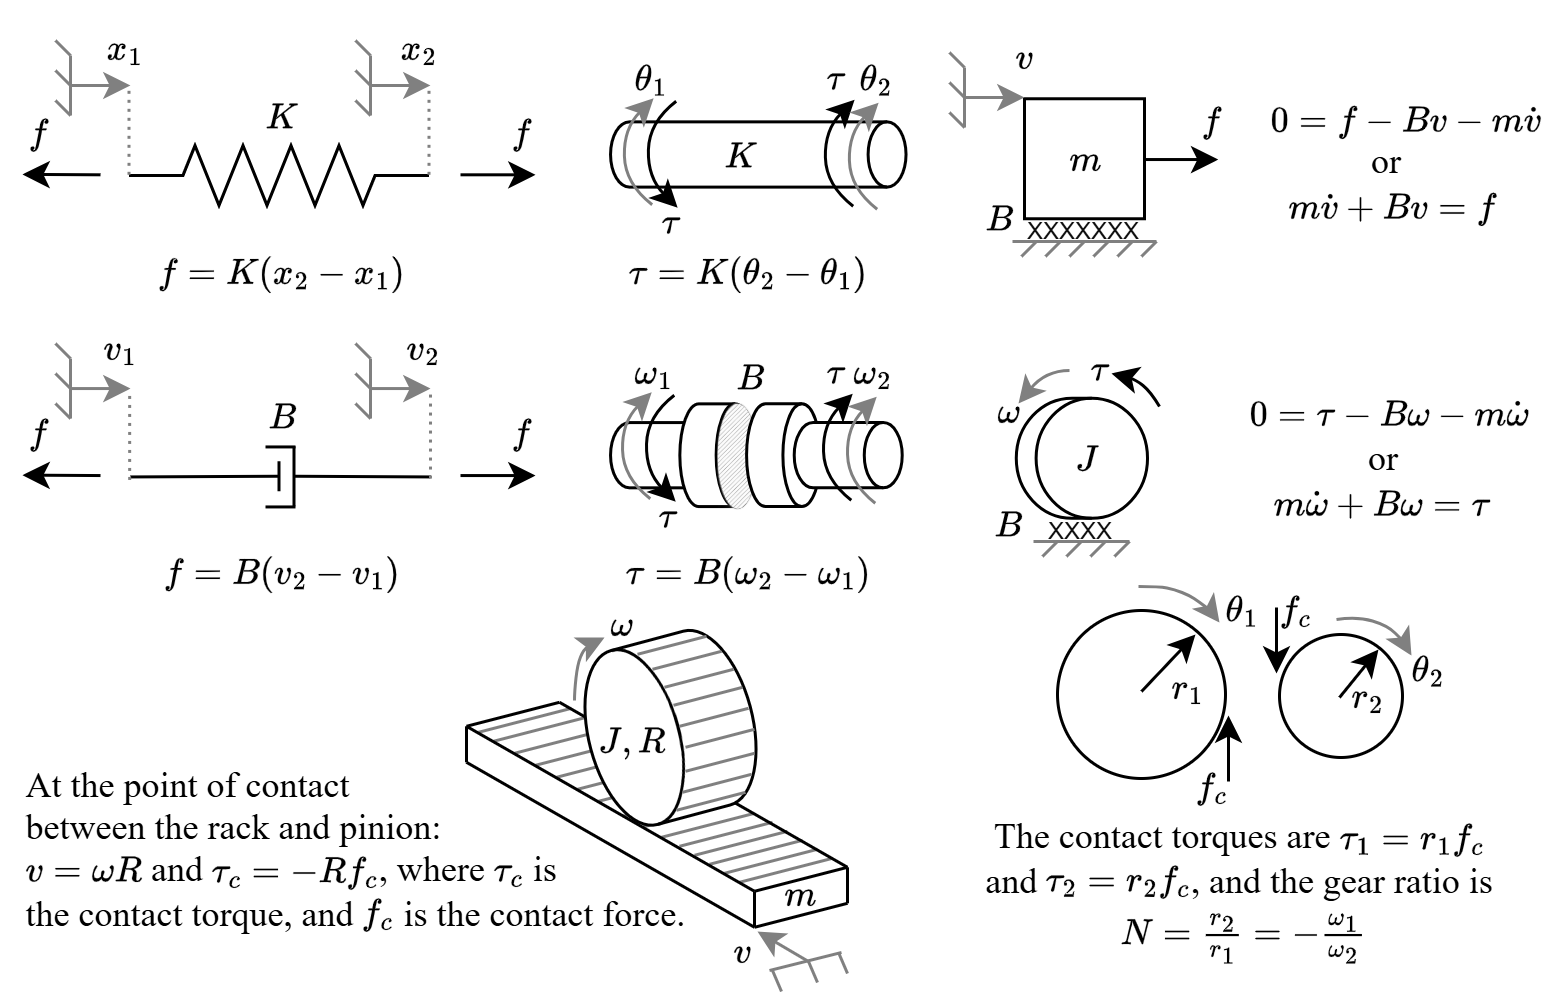
\includegraphics[width=\linewidth]{figures/mechanical_schematics.png}
\end{figure}\\
\noindent\textbf{\underline{Electrical Circuits:}}
\begin{figure}[h]    
    \centering            
    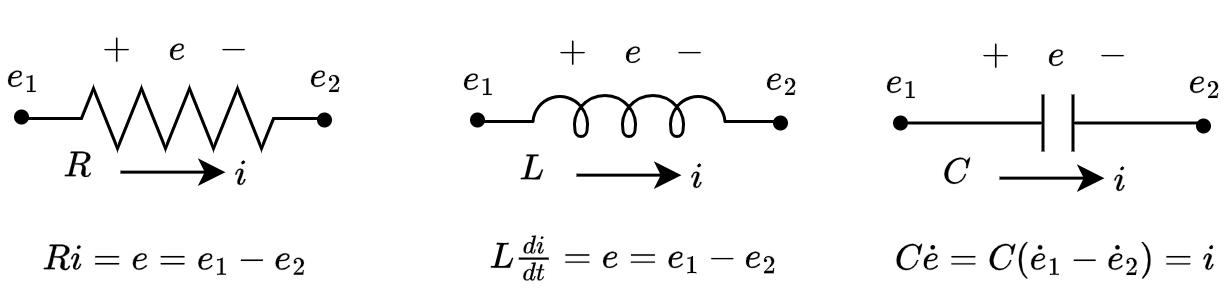
\includegraphics[width=0.825\linewidth]{figures/electrical_schematics.png}
\end{figure}\\
\begin{minipage}{0.45\linewidth}
    \noindent\underline{Ideal Operational Amplifier Rules:}
    \begin{enumerate}
        \item No current flow at the \(+\) or \(-\) terminals.
        \item When the output terminal has a feedback connection to the \(-\) terminal, \(e_+ = e_-\).
    \end{enumerate}
\end{minipage}
\begin{minipage}{0.5\linewidth}
    \centering
    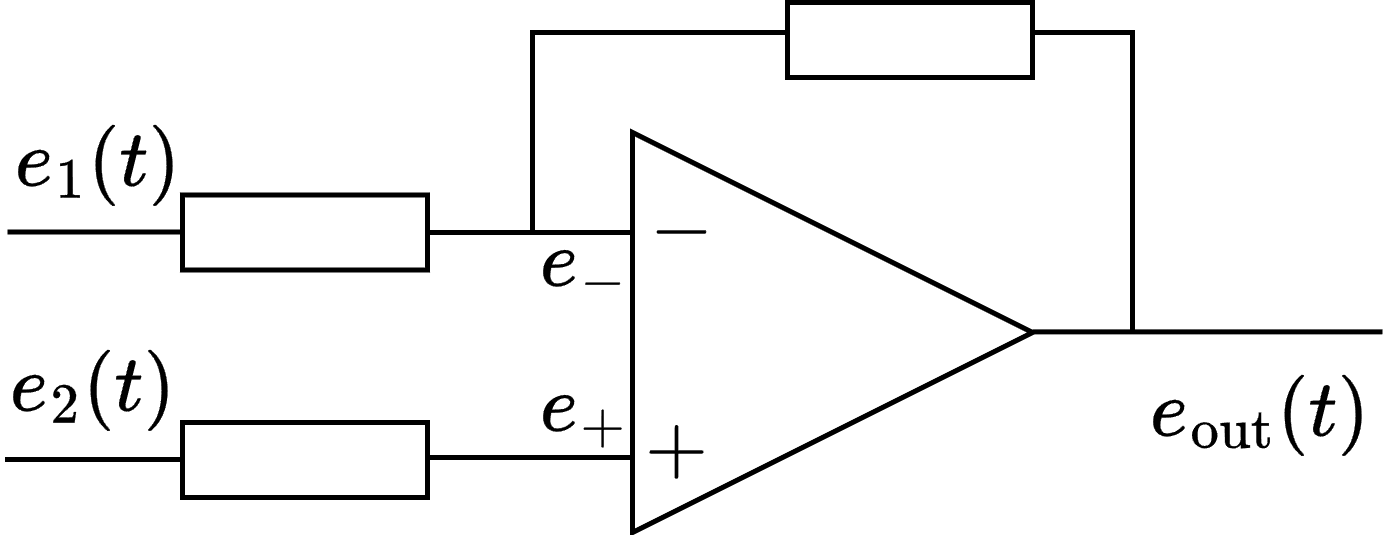
\includegraphics[width=0.75\linewidth]{figures/ideal_op_amp.png}
\end{minipage}\\

\noindent\textbf{\underline{State Space Form:}}\\
For a system with \(n\) states, \(m\) inputs, and \(p\)  outputs, the state-space form is \(\begin{cases} \dot{\bm{x}}(t) = \bm{A}\bm{x}(t) + \bm{B}\bm{u}(t)\\    \bm{y}(t) = \bm{C}\bm{x}(t) + \bm{D}\bm{u}(t) \end{cases}\)
where \(\bm{A}\) is \(n\times n\), \(\bm{B}\) is \(n\times m\), \(\bm{C}\) is \(p\times n\), and \(\bm{D}\) is \(p\times m\).

\noindent\textbf{\underline{Linearization:}}\\
The incremental variables \(\hat{x}(t) = x(t) - \overline{x}\) and \(\hat{f}(t) = f(t) -\overline{f}\) linearize a system at the operating point \((\overline{x},\, \overline{f})\). A nonlinear function \(y(t) = f(x(t))\) may be linearized as \(y(t) \approx f(\overline{x}) + \dfrac{\partial f}{\partial x}\bigg|_{\overline{x}}\hat{x}(t)\).


\noindent\textbf{\underline{First-Order and Second-Order Systems:}}
\begin{itemize}
    \item First-order ODE standard form: \(\dot{y}(t) + ay(t) = Ku(t)\), where \(\tau = 1/a\) is the time constant.
    \item Second-order ODE standard form: \(\ddot{x}(t) + 2\zeta\omega_n \dot{x}(t)  + \omega_n^2x(t) = K\omega_n^2u(t)\), where \(\zeta\) is the damping ratio, and \(\omega_n \geq0\) is the natural frequency.
    \item For a bounded time-domain function \(g(t)\), with Laplace transform \(G(s) = \mathcal{L}\{g(t)\}\):
    \begin{itemize}
        \item Final value theorem: \(g(\infty) = \displaystyle\lim_{t\to\infty} g(t)  = \displaystyle\lim_{s\to0} sG(s)\)
        \item Initial value theorem: \(g(0^+) = \displaystyle\lim_{t\to0^+} g(t) = \displaystyle\lim_{s\to\infty} sG(s)\)
    \end{itemize}
    \item Settling time: \(T_s = 5\tau = -5/\sigma\), where \(\sigma\) is the real part of the pole that is the closest to the \(j\omega\)-axis.
    \item With zero initial-conditions, when a step-input is applied, a generic second-order step-response is \\
    \begin{minipage}{0.6\linewidth}
        \centering
        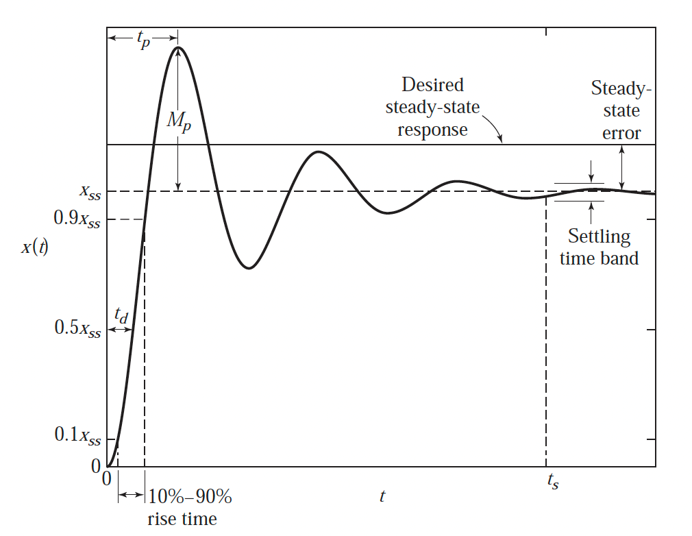
\includegraphics[width=0.95\linewidth]{figures/second_order_step_response.png}
    \end{minipage}
    \begin{minipage}{0.3\linewidth}
        \vfill
        where:
        \begin{align*}            
            M_p &= e^{\left(\frac{-\pi\zeta}{\sqrt{1-\zeta^2}}\right)}\\
            &\\
            T_p &= \dfrac{\pi}{\omega_n\sqrt{1-\zeta^2}} = \dfrac{\pi}{\omega_d}\\
            &\\
            \%O.S. &= e^{\left(\frac{-\zeta\pi}{\sqrt{1-\zeta^2}}\right)} \times 100\% \\            
        \end{align*}
        \vfill
    \end{minipage}
\end{itemize}


\noindent\textbf{\underline{Partial Fraction Expansion:}}\\
In each applicable case, \(a\), \(A\), \(B\), and \(C\) are real-valued numbers.
\begin{itemize}
    \item Distinct and real roots: \emph{e.g.}, \(F(s) = \dfrac{1}{(s+\sigma_1)(s+\sigma_2)} = \dfrac{A}{s+\sigma_1} + \dfrac{B}{s+\sigma_2}\)
    \item Repeated real roots: \emph{e.g.}, \(F(s) = \dfrac{1}{(s+\sigma_1)^2} = \dfrac{A}{(s+\sigma_1)^2} + \dfrac{B}{s+\sigma_1}\)
    \item Complex roots: \emph{e.g.}, \(F(s) = \dfrac{s+z}{(s+\sigma -j\omega)(s+\sigma +j\omega)} = \dfrac{s+z}{s^2 +2\sigma s +\omega^2} = \dfrac{Bs+ C}{(s+a)^2 + \omega^2}\)
\end{itemize}
\noindent\textbf{\underline{Common Moments of Inertia:}}
\begin{figure}[H]
    \centering
    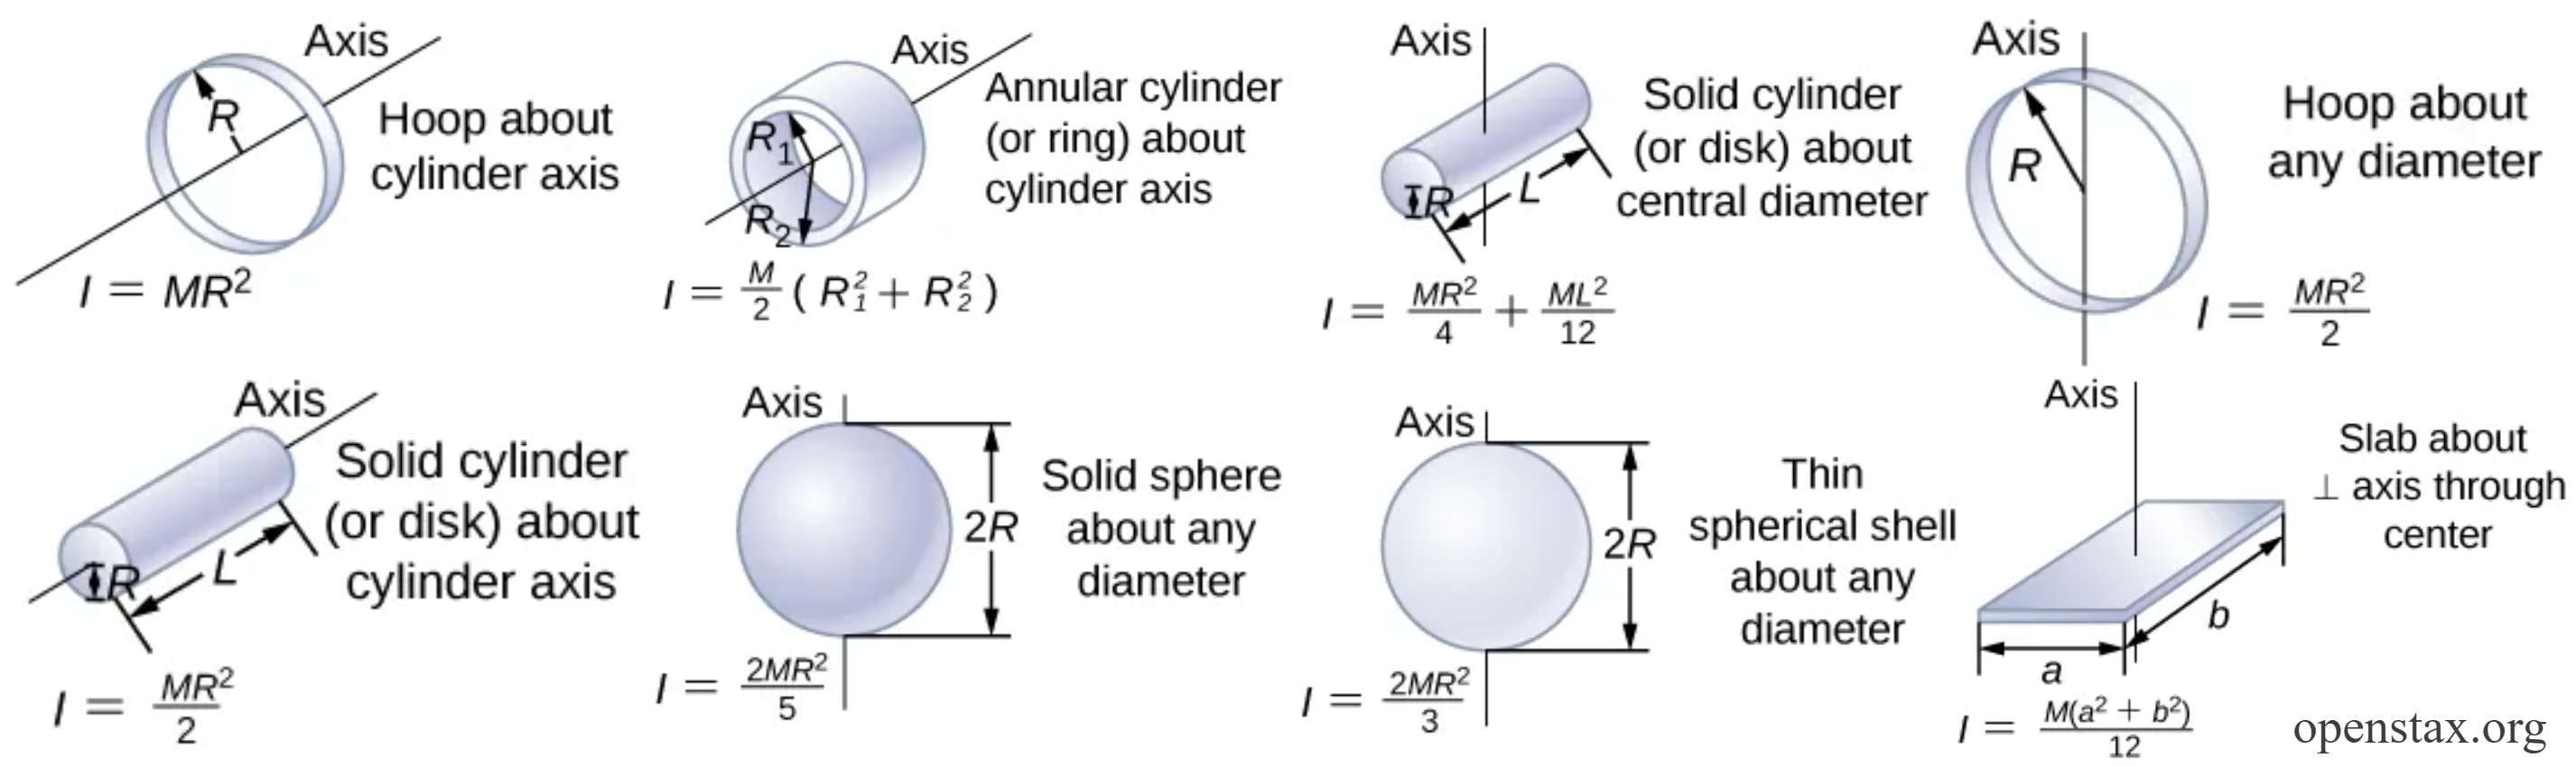
\includegraphics[width=\linewidth]{figures/openstax_moi_table_modified.png}
\end{figure}

\newpage
\noindent\textbf{\underline{Permanent Magnet Brushed DC Motors:}}\\
\begin{minipage}{0.45\linewidth}
    \noindent \underline{Electrical Portion:}\\
    Applied voltage \(e_a(t)\), resistance \(R\),\\inductance \(L\), back-emf constant \(k_e=k_\tau\)\\

    \noindent \underline{Mechanical Portion:}\\
    Applied torque \(\tau_a(t)\), rotational inertia \(J\),\\damping \(B\), torque constant \(k_\tau = k_e\)
\end{minipage}
\hfill
\begin{minipage}{0.5\linewidth}    
    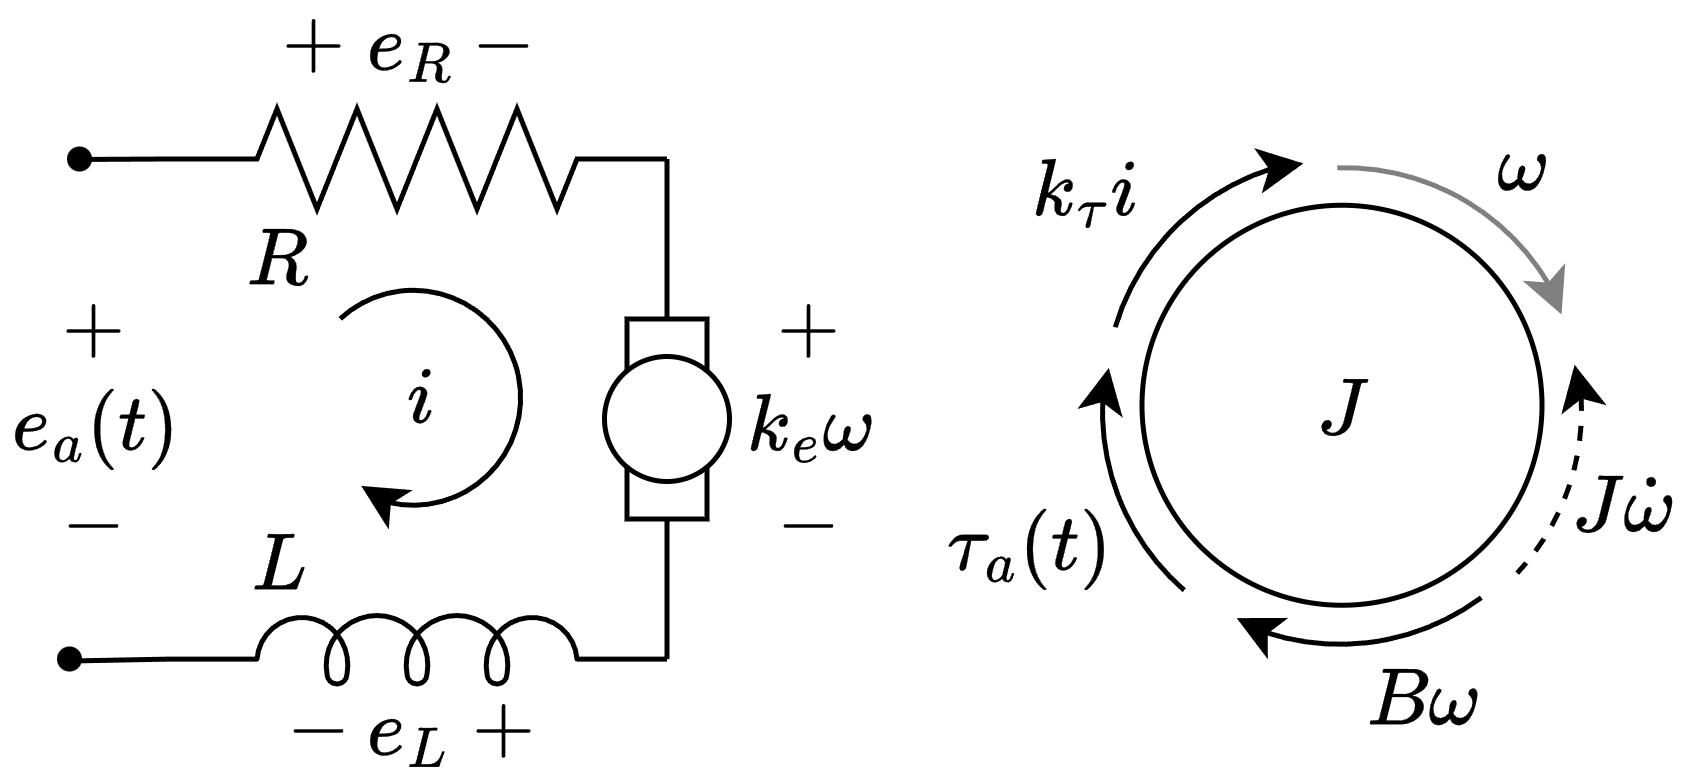
\includegraphics[width=\linewidth]{figures/dc_motor.png}
\end{minipage}

\noindent\textbf{\underline{Controlled Systems:}}\\
For the block diagram shown, it has output \(Y(s)\), reference \(R(s)\), controller transfer function \(C(s)\), uncontrolled physical plant transfer function \(G_p(s)\), and sensor transfer function \(H(s)\).\\
\begin{figure}[H]
    \centering
    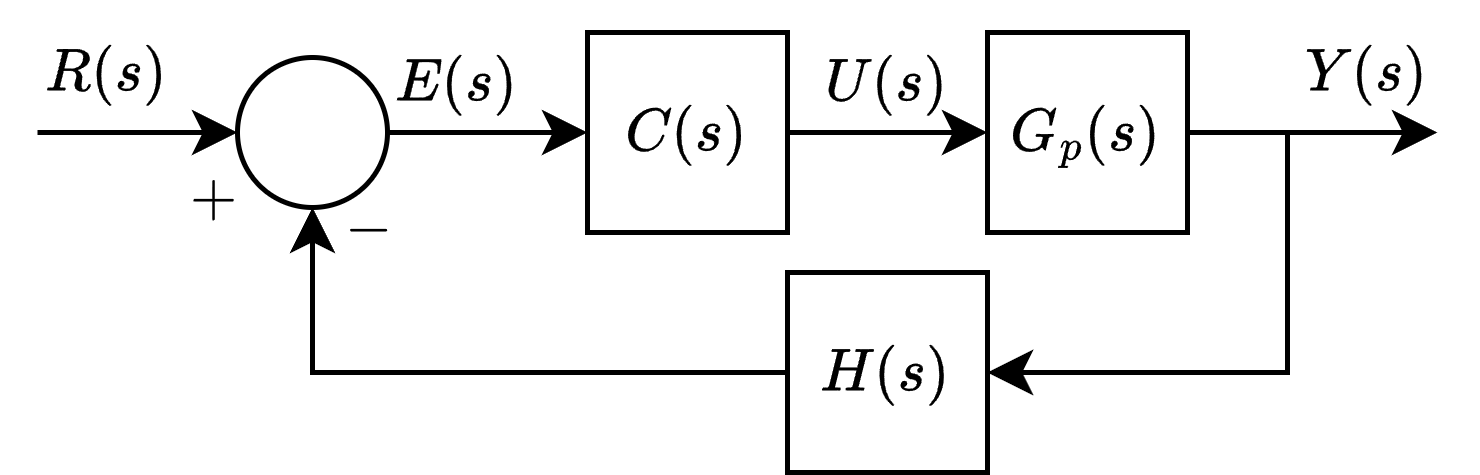
\includegraphics[width=0.5\linewidth]{figures/controlled_system.png}
\end{figure}        
\begin{itemize}
    \item Its closed-loop transfer function is \(G_{CL}(s) = \dfrac{Y(s)}{R(s)}\) \(= \dfrac{C(s)G_p(s)}{1+ H(s)C(s)G_p(s)}\).
    \item Its open-loop transfer function is \(KG(s) = H(s)C(s)G_p(s)\), where \(K\) is the DC-gain of the system.
    \item Its closed-loop characteristic equation is \(0 = 1 + H(s)C(s)G_p(s))\). Thus, \(KG(s) = -1\).
\end{itemize}
For PID control: \(C(s) = K_p + K_i\dfrac{1}{s} + sK_d\) and \(u(t) = K_pe(t) + K_i \displaystyle\int e(t)dt + K_d\dfrac{d}{dt}e(t)\).        

\noindent\textbf{\underline{Root Locus:}}\\
The governing equation is \(1 + K^*L(s) = 0\).
\begin{enumerate}[label=(\alph*)]
    \item Root locus begins at the (open-loop) poles, and ends at the (open-loop) zeroes.
    \item The number of branches equals the number of open-loop poles.
    \item The root locus plot is symmetrical about the real-axis.
    \item Real-axis segments are to the left of the odd numbered real-axis finite open-loop poles and zeroes.
    \item When there are more poles than zeroes, the extra branches will each approach an asymptote. These asymptote(s) have centroid \(\sigma_a = \dfrac{\sum_{j=1}^n p_j - \sum_{i=1}^m z_i}{n-m}\) (\emph{i.e.}, the intersection point of all asymptotes on the real axis), and angles \(\theta_a =\dfrac{(2k+1)\pi}{n-m}\), for \(k =0,\,1,\, \cdots,\, n-m-1\).
    \item The real-axis break-in and break-away points can be found by setting \(K^*(s) = \dfrac{-1}{L(s)}\), and solving \(\dfrac{dK^*(s)}{ds} = 0\), for real values of \(s\). Or, by writing the open-loop transfer function \(K^*L(s) = K^*\dfrac{N(s)}{D(s)}\), and solving for the value(s) of \(s\) that satisfy \(\dfrac{dD(s)}{ds}N(s) - D(s)\dfrac{dN(s)}{ds} = 0\).
    \item The imaginary-axis crossing (\emph{i.e.}, transition to instability) can be found by setting \(K^*L(j\omega) = -1\), and solving for the values of \(\omega\) that satisfy \(\operatorname{Re}\{L(s)\} = -1\) and \(\operatorname{Im}\{L(s)\} = 0\).
\end{enumerate}        

\newpage
\vfill
\renewcommand{\arraystretch}{2.5}
\begin{table}
    \centering
    \caption{Transforms of Functions}
    \begin{tabular}{ll}
        \toprule
        \vspace{-50pt}\\
        \textbf{Time Functions} & \textbf{Transformed Functions}\\
        \vspace{-42.5pt}\\
        \midrule
        \(\delta(t)\) & \(1\)\\
        \(U(t)\) & \(\dfrac{1}{s}\)\\ 
        \(A\) & \(\dfrac{A}{s}\)\\
        \(t\) & \(\dfrac{1}{s^2}\)\\
        \(t^2\) & \(\dfrac{2!}{s^3}\)\\
        \(t^n\) for \(n = 1,\,2,\,3,\,\dots\) &  \(\dfrac{n!}{s^{n+1}}\)\\
        \(e^{-at}\) & \(\dfrac{1}{s+a}\)\\
        \(te^{-at}\) & \(\dfrac{1}{(s+a)^2}\)\\
        \(t^2e^{-at}\) & \(\dfrac{2!}{(s+a)^3}\)\\
        \(\sin(\omega t)\) & \(\dfrac{\omega}{s^2+\omega^2}\)\\
        \(\cos(\omega t)\) & \(\dfrac{s}{s^2+\omega^2}\)\\
        \(e^{-at}\sin(\omega t)\) & \(\dfrac{\omega}{(s+a)^2+ \omega^2}\)\\
        \(e^{-at}\cos(\omega t)\) & \(\dfrac{s+a}{(s+a)^2 + \omega^2}\)\\
        \(e^{-at}\left[B\cos(\omega t) + \left(\dfrac{C-aB}{\omega}\right)\sin(\omega t) \right]\) \hspace{10pt} & \(\dfrac{Bs + C}{(s+a)^2 + \omega^2}\)\\
        \(2Ke^{-at}\cos(\omega t  + \phi)\) & \(\dfrac{Ke^{j\phi}}{s+a-j\omega} + \dfrac{Ke^{-j\phi}}{s+a+j\omega}\)\\
        \bottomrule
    \end{tabular}        
\end{table}
\vfill

\newpage
\vfill
\begin{table}
    \centering
    \caption{Transform Properties}
    \begin{tabular}{ll}
         \toprule
         \vspace{-50pt}\\
         \textbf{Time functions} & \textbf{Transformed functions}\\
         \vspace{-40pt}\\
         \hline
         \(f(t)\) & \(F(s)\)\\
         \(af(t)\) & \(aF(s)\)\\
         \(f(t) + g(t)\) & \(F(s) + G(s)\)\\
         \(e^{-at}f(t)\) & \(F(s+a)\)\\
         \(tf(t)\) & \(-\dfrac{d}{ds}F(s)\)\\
         \(f(t/a)\) & \(aF(as)\)\\
         \(\left[f(t-a)\right]U(t-a)\) & \(e^{-sa}F(s)\)\\
         \(\dot{f}(t)\) & \(sF(s) - f(0)\)\\
         \(\ddot{f}(t)\) & \(s^2F(s) - sf(0) - \dot{f}(0)\)\\
         \(\dddot{f}(t)\) & \(s^3F(s) - s^2f(0) - s\dot{f}(0) -\ddot{f}(0)\)\\
         \(\dfrac{d^nf}{dt^n}\) for \(n=1,\,2,\,3,\,\dots\) \hspace{10pt} & \(s^nF(s) -s^{n-1}f(0) - \cdots - sf^{(n-2)}(0) - f^{(n-1)}(0)\)\\
         \(\displaystyle\int_0^tf(\lambda) d\lambda\) & \(\dfrac{1}{s}F(s)\)\\        
         \(f(0^+)\) & \(\displaystyle\lim_{s\to\infty} sF(s)\)\\
         \(f(\infty)\) & \(\displaystyle\lim_{s\to0} sF(s)\)\\
         \bottomrule
    \end{tabular}        
\end{table}
\vfill


\end{document}